\section{FFF circuit with two input nodes}
\label{sec:fff}

The diagram of this circuit is shown at Fig.~\ref{fig:twoinput_fff}.

\begin{figure}[H]
    \centering
    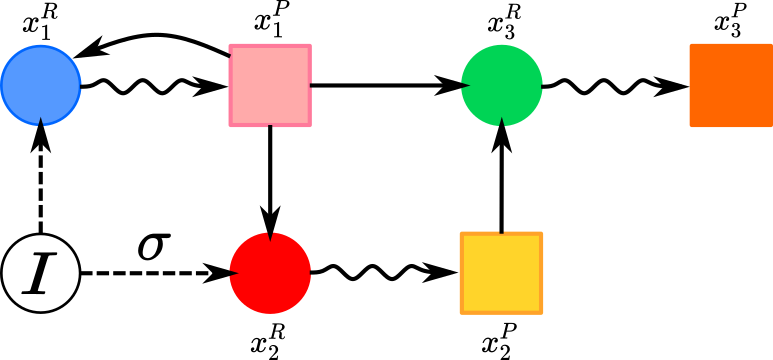
\includegraphics[scale=0.7]{figs/broken_n1_1.png}
    \caption{Feed-Forward Fiber circuit with two input nodes 
    ($x_1^R$ and $x_2^R$) and output node $x_3^P$.}
    \label{fig:twoinput_fff}
\end{figure}

The special model \cite{stochs_gene_2005,homeostasis_antonelli2018} used for this circuit is given by the set 
of nonlinear differential equations of Eq.~\ref{eq:special_fff}:
\begin{equation} \label{eq:special_fff}
    \begin{aligned} 
        f_{x_1^R}(x_1^R, x_1^P, \mathcal{I}) &= -\delta x_1^R + \gamma\tilde{f}(x_1^P) + \mathcal{I}\\ 
        f_{x_1^P}(x_1^P, x_1^R) &= -\alpha x_1^P + \beta x_1^R \\ 
        f_{x_2^R}(x_2^R, x_1^P, \mathcal{I}) &= -\delta x_2^R + \gamma\tilde{f}(x_1^P) + \sigma \mathcal{I} \\
        f_{x_2^P}(x_2^P, x_2^R) &= -\alpha x_2^P + \beta x_2^R   \\
        f_{x_3^R}(x_3^R, x_1^P, x_2^P) &= -\delta x_3^R + \gamma \tilde{g}(x_1^P,x_2^P) \\
        f_{x_3^P}(x_3^P, x_3^R) &= -\alpha x_3^P + \beta x_3^R
    \end{aligned},
\end{equation}
where $\tilde{f}$ and $\tilde{g}$ are monotonic nonlinear functions within the interval $[0,1]$. 
Specifically, $\tilde{f}$ and $\tilde{g}$ are defined as Hill functions,
and $\tilde{g}(x_1^P, x_2^P) = \tilde{g}(x_1^P + x_2^P)$.

The general infinitesimal homeostasis condition obtained by using the algorithm of 
\cite{multi_input_antoneli2020}, which is a generalization of \cite{wang2021} for multiple inputs, 
is given by Eq.~\ref{eq:gen_inf_hom} below:
\begin{equation} \label{eq:gen_inf_hom}
    \begin{split}
    &+f_{x_2^R, I}f_{x_2^P, x_2^R}f_{x_3^R, x_2^P}(f_{x_1^R, x_1^R}f_{x_1^P, x_1^P} - f_{x_1^R,x_1^P}f_{x_1^P, x_1^R}) \\ 
    &+f_{x_1^R, I}f_{x_1^P,x_1^R}(f_{x_2^R, x_1^P}f_{x_2^P, x_2^R}f_{x_3^R, x_2^P} + f_{x_2^R, x_2^R}f_{x_2^P, x_2^P}f_{x_3^R, x_1^P}) = 0
    \end{split},
\end{equation}
which is translated to Eq.~\ref{eq:special_inf_hom} according to Eq.~\ref{eq:special_fff} as:
\begin{equation} \label{eq:special_inf_hom}
    \tilde{g}'(x_1^P + x_2^P) \bigg\{ \alpha \delta (1+\sigma) + \gamma \beta \tilde{f}'(x_1^P)(1-\sigma) \bigg\} = 0.
\end{equation}

From condition of Eq.~\ref{eq:special_inf_hom}, we can determine the relations 
to be satisfied together with the additional conditions for infinitesimal chair at some
input value $\mathcal{I}_0$. Thus, we can state that a stable equilibrium $\vec{x}_{\infty}$
at $\mathcal{I}_0$ satisfies the infinitesimal homeostasis condition, 
$x_{3(\infty),\mathcal{I}}^P(\mathcal{I}_0) = 0$, iff
\begin{equation} \label{eq:special_inf_hom_rho}
    \rho(\mathcal{I}_0) \equiv \tilde{g}'(x_1^P + x_2^P) \bigg\{ \alpha \delta (1+\sigma) + \gamma \beta \tilde{f}'(x_1^P)(1-\sigma) \bigg\} = 0,
\end{equation}
and an infinitesimal chair point occurs if, according to the same assumptions, we satisfy the additional
conditions
\begin{equation}
    \frac{d\rho}{d\mathcal{I}}(\mathcal{I}_0) = 0 \ \text{ and } \ \frac{d^2\rho}{d\mathcal{I}^2}(\mathcal{I}_0) \neq 0.
\end{equation}

Following each one of the four conditions described above (equilibrium, infinitesimal homeostasis
and the two conditions for infinitesimal chair), we can obtain the relations shown in 
Eq.~\ref{eq:gen-special-rel} below:
\begin{equation} \label{eq:gen-special-rel}
    \begin{aligned} \tilde{f}(x_1^P) &= \frac{\alpha \delta}{\beta \gamma}x_1^P - \frac{\mathcal{I}_0}{\gamma} \\
    \tilde{f}'(x_1^P) &= - \frac{\alpha\delta}{\beta\gamma}\frac{(1+\sigma)}{(1-\sigma)} \\ 
    \tilde{f}&''(x_1^P) = 0 \\ 
    \tilde{f}&'''(x_1^P) \neq 0  
    \end{aligned},
\end{equation}
for $\sigma \neq 1$. Again, $\tilde{f}$ is either an increasing or decreasing monotonic 
nonlinear function within the interval $[0,1]$ represented by a Hill function of exponent $n$. 
Note that from the second condition to the fourth, we assume that the 
homeostasis behavior is reached by considering that the second term of $\rho(\mathcal{I}_0)$
is zero. Thus, at first we ignore the possibility of $\tilde{g}'(x_1^P + x_2^P) = 0$, which 
happens only for total degradation ($x_1^P(\mathcal{I}) + x_2^P(\mathcal{I}) = 0$) or asymptotic saturation
through $x_1^P(\mathcal{I}) + x_2^P(\mathcal{I}) \rightarrow \infty$, where $\infty$ only means that the
sum is large enough to satisfy $\tilde{g}'(x_1^P + x_2^P) = 0$.

% specify the function.
In order to perform numerical tests, we specify the form of $\tilde{f}$ and $\tilde{g}$
according to a Hill function $S(x)$(or $S(x+y)$ for $\tilde{g}$) of exponent $n = 2$.
This way, we have 
\begin{equation} \label{eq:hill2}
    S(x) = \frac{1}{1+x^2} \ \ \ \text{and} \ \ \ S(x+y) = \frac{1}{1+(x+y)^2},
\end{equation}
from which we list the following derivatives:
\begin{equation} \label{eq:s-derivatives}
    \begin{aligned}
        S'(x) &= -\frac{2x}{(1+x^2)^2} \\
        S''(x) &= -\frac{2(1-3x^2)}{(1+x^2)^3}\\
        S'''(x) &= \frac{24x(1-x^2)}{(1+x^2)^4}
    \end{aligned}.
\end{equation}

\subsection{Case 1: $\tilde{f}(x) \equiv S(x)$ - UNSAT-FFF}

By defining $\tilde{f} \equiv S(x)$, we consider that all regulations within the fiber 
(between nodes $x_1^R, x_1^P, x_2^R, x_2^P$) are repressors, which defines the 
UNSAT feed-forward fiber \cite{transistor2019}. For this circuit the conditions 
defined in Eq.~\ref{eq:gen-special-rel} is translated to conditions of
Eq.~\ref{eq:unsat-conditions}: 
\begin{equation} \label{eq:unsat-conditions}
    \begin{aligned}
        S(x_1^P) &= \frac{\alpha \delta}{\beta \gamma}x_1^P - \frac{\mathcal{I}_0}{\gamma} \\
        S'(x_1^P) &= - \frac{\alpha\delta}{\beta\gamma}\frac{(1+\sigma)}{(1-\sigma)} \\
        S&''(x_1^P) = 0\\
        S&'''(x_1^P) \neq 0
    \end{aligned}.
\end{equation}
Now, from Eq.~\ref{eq:unsat-conditions} and using the specific form of $S$ and its 
derivatives displayed in Eq.~\ref{eq:s-derivatives}, we perform further calculations to 
obtain the expression for $\mathcal{I}_0$. 

From $S''(x_1^P) = 0$, we have that $x_{1(\infty)}^P(\mathcal{I}_0) = 1/\sqrt{3}$. $x_{1(\infty)}^P$ is
the protein concentration 1 at the stable equilibrium $\vec{x}_{\infty}$. Then,
from the equilibrium condition we obtain the expression for $\mathcal{I}_0$ in terms of the
parameters of the special model:
\begin{equation} \label{eq:Io-param-unsat}
    \mathcal{I}_0 = \gamma\Bigg(\frac{\alpha \delta}{\beta \gamma}\frac{1}{\sqrt{3}} - \frac{3}{4}\Bigg),
\end{equation} 
which can be simplified by using the second condition and using $S'(x_{1(\infty)}^P) = -3\sqrt{3}/8$:
\begin{equation}
    \frac{\alpha \delta}{\beta \gamma} = \frac{3\sqrt{3}}{8}\frac{(1-\sigma)}{(1+\sigma)},
\end{equation}
and finally we have the final form for the infinitesimal homeostasis point:
\begin{equation} \label{eq:Io-sigma-unsat}
    \mathcal{I}_0 = \gamma\Bigg(\frac{3}{8}\frac{(1-\sigma)}{(1+\sigma)} - \frac{3}{4}\Bigg).
\end{equation}
Concerning $\tilde{g}(x_1^P + x_2^P)$, its specific form should influence only the set point 
defined by $x_{3(\infty)}^P$, but not at which value the homeostasis point $\mathcal{I}_0$  should occur
(However, if $x_1^P$ and $x_2^P$ provides different regulations to $x_3^P$, we cannot represent 
$\tilde{g}(x_1^P, x_2^P)$ as $\tilde{g}(x_1^P + x_2^P)$ as showed in Eq.~\ref{eq:hill2}). We can 
also find relations for allowed values of $\sigma$ considering the nonnegative model parameters 
and allowed values of $\mathcal{I}$, but for now we only make these relations explicit during 
the numerical tests (Fig.~\ref{fig:unsat_ex1} and Fig.~\ref{fig:unsat_ex1-1}).

\begin{figure}[H]
    \centering
    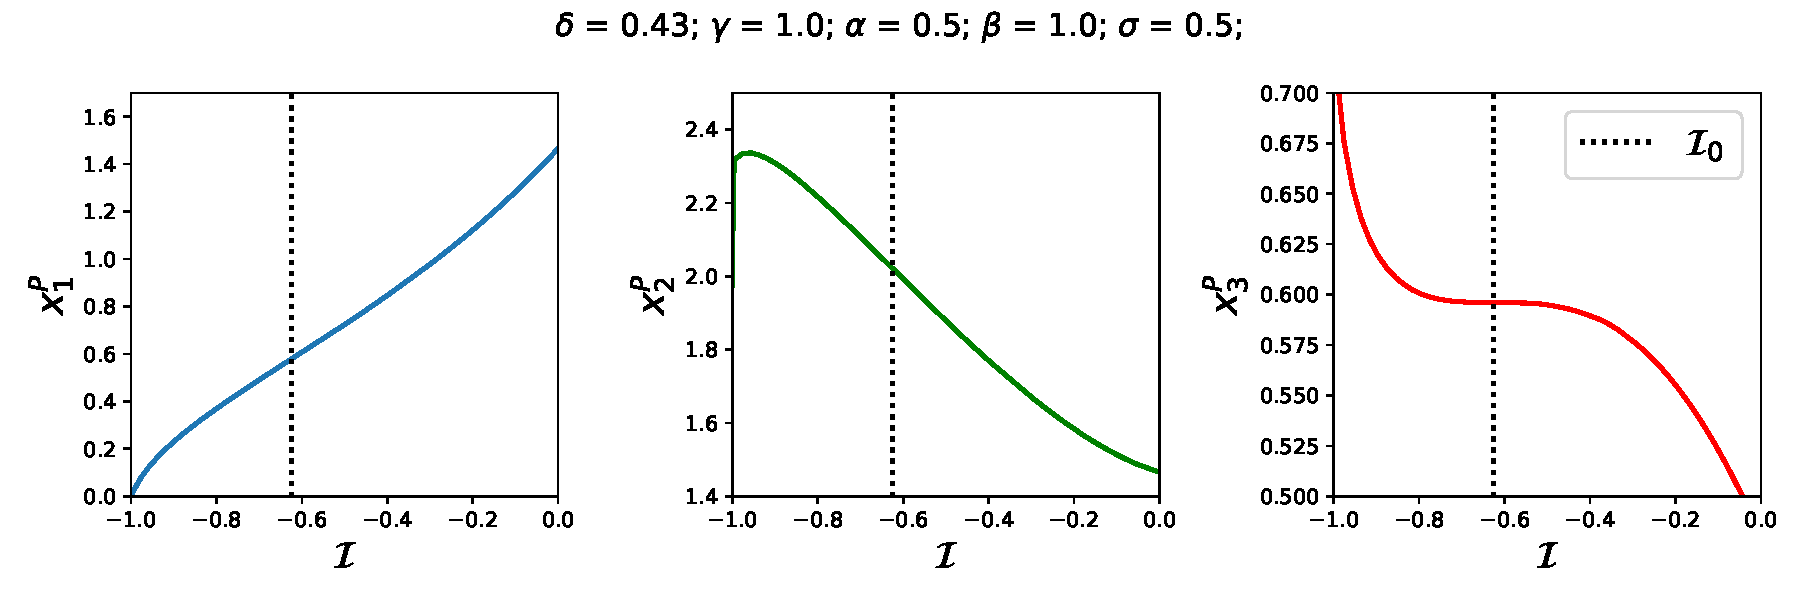
\includegraphics[scale=0.5]{figs/numerics/unsatfff_twoinput_1.pdf}
    \caption{$\tilde{f}(x_1^P) \equiv S(x_1^P)$ and $\tilde{g}(x_1^P + x_2^P) \equiv S(x_1^P + x_2^P)$.}
    \label{fig:unsat_ex1}
\end{figure}

\begin{figure}[H]
    \centering
    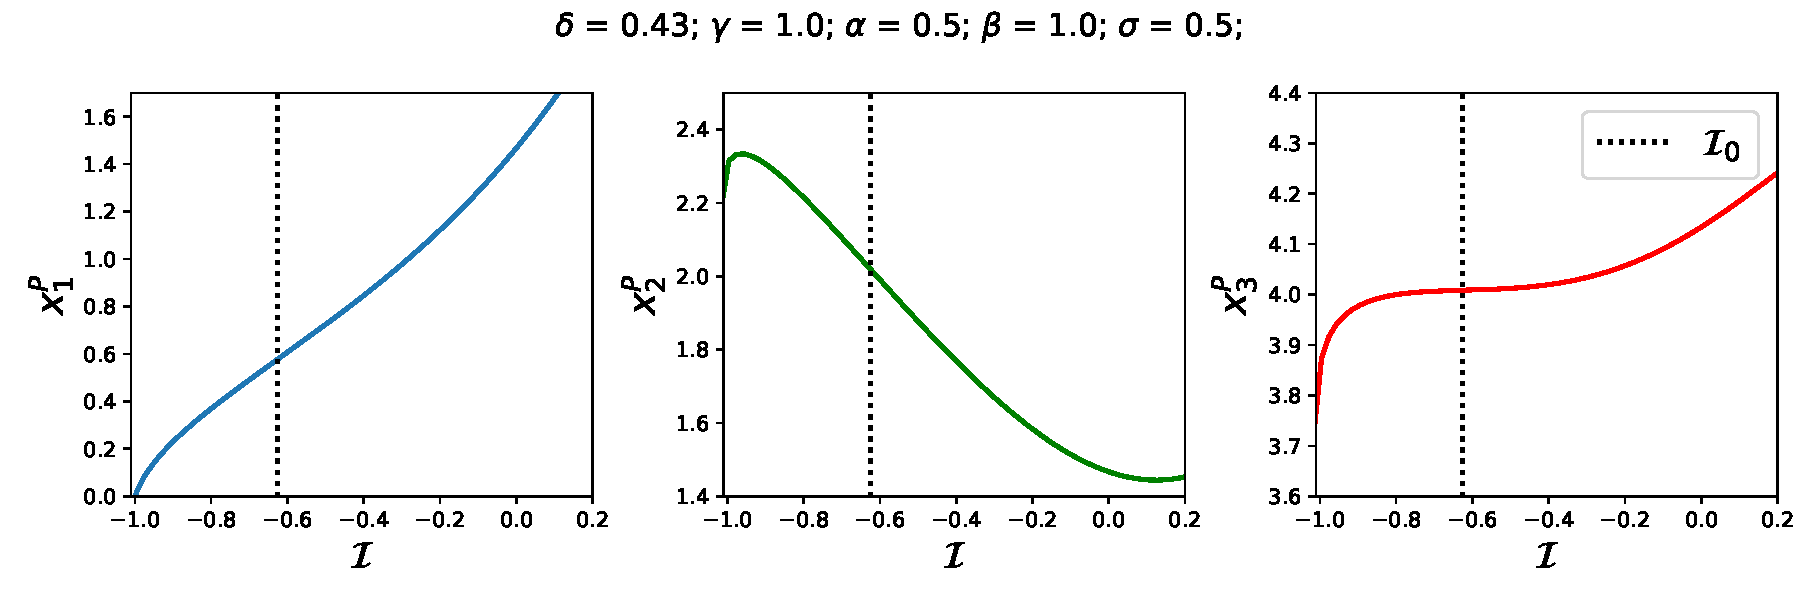
\includegraphics[scale=0.5]{figs/numerics/unsatfff_twoinput_2.pdf}
    \caption{$\tilde{f}(x_1^P) \equiv S(x_1^P)$ and $\tilde{g}(x_1^P + x_2^P) \equiv 1 - S(x_1^P + x_2^P)$.}
    \label{fig:unsat_ex1-1}
\end{figure}

\subsection{Case 2: $\tilde{f}(x) \equiv 1 - S(x)$ - SAT-FFF}

By defining $\tilde{f} \equiv 1 - S(x)$, we consider that all regulations within the fiber 
(between nodes $x_1^R, x_1^P, x_2^R, x_2^P$) are activators, which defines the 
SAT feed-forward fiber \cite{transistor2019}. For this circuit the conditions 
defined in Eq.~\ref{eq:gen-special-rel} is translated to the relations of
Eq.~\ref{eq:sat-conditions}: 
\begin{equation} \label{eq:sat-conditions}
    \begin{aligned} S(x_1^P) &= -\frac{\alpha \delta}{\beta \gamma}x_1^P + \big(1+ \frac{\mathcal{I}_0}{\gamma}\big) \\ 
        S'(&x_1^P) = \frac{\alpha\delta}{\beta\gamma}\frac{(1+\sigma)}{(1-\sigma)} \\ 
        &S''(x_1^P) = 0 \\ 
        &S'''(x_1^P) \neq 0  
    \end{aligned}.
\end{equation}
Assuming that the second term of Eq.~\ref{eq:special_inf_hom} is zero at $\mathcal{I}_0$, 
we can proceed with the calculations similarly as the UNSAT-FFF case before. Thus, 
following the conditions above, we obtain $x_{1(\infty)}^P = 1/\sqrt{3}$ for the stable 
equilibrium just as in the UNSAT-FFF case. From $S'(x_{1(\infty)}^P)$, we obtain the relation
\begin{equation}
    \frac{\alpha \delta}{\beta \gamma} = - \frac{3\sqrt{3}}{8}\frac{(1-\sigma)}{(1+\sigma)},
\end{equation} 
from which we obtain the expression for the infinitesimal homeostasis point
\begin{equation}
        \mathcal{I}_0 = -\gamma\bigg(\frac{3}{8}\frac{(1-\sigma)}{(1+\sigma)} + \frac{1}{4}\bigg).  
\end{equation}
Therefore, these conditions should be satisfied if $\rho(\mathcal{I}_0) = 0$ through its second 
term, meaning that $\tilde{g}'(x_1^P(\mathcal{I}) + x_2^P(\mathcal{I})) \neq 0$.

However, from what it is observed from the numerical calculations, these conditions are 
not fulfilled for positive regulations. We now show some of the numerical results obtained for the SAT-FFF and 
after we explain how the homeostasis is obtained for this circuit.

\begin{figure}[H]
    \centering
    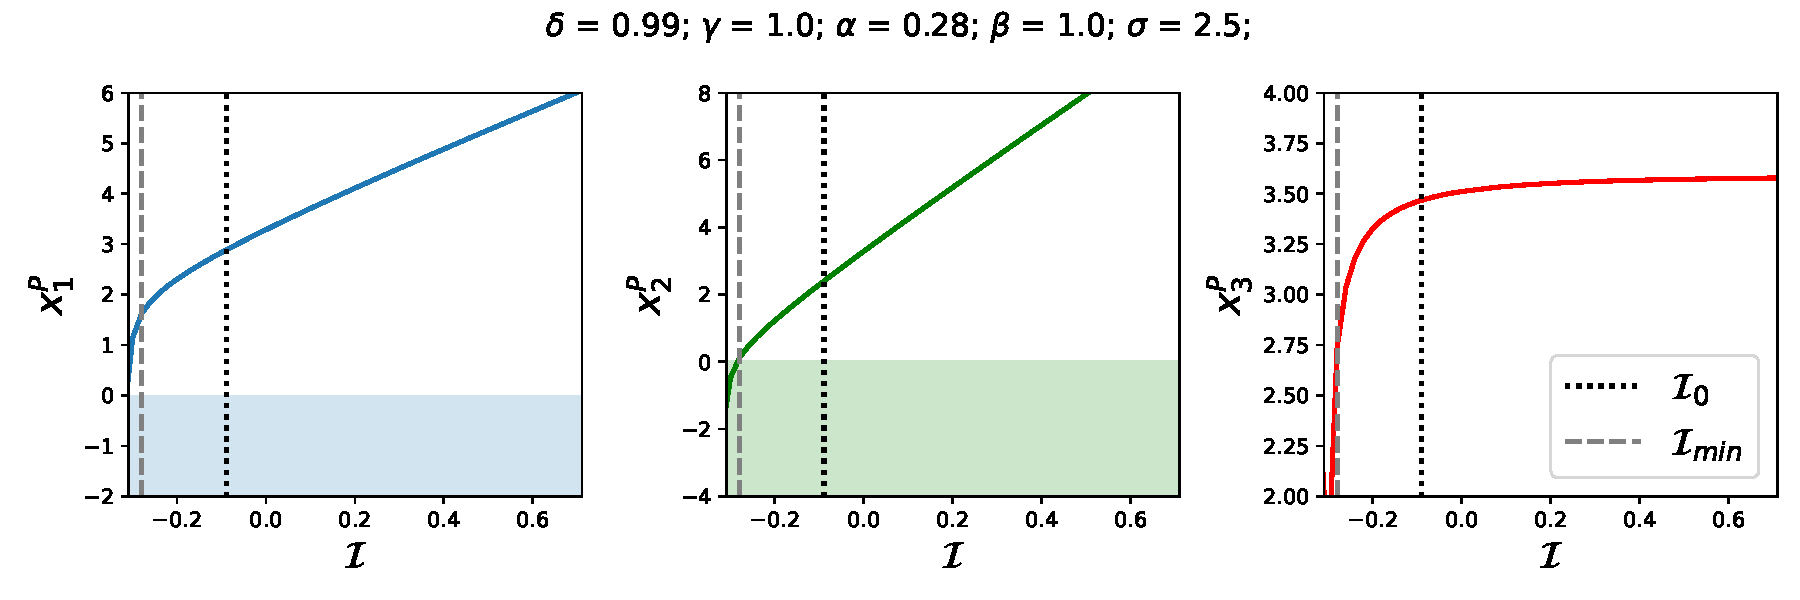
\includegraphics[scale=0.5]{figs/numerics/satfff_twoinput_ex1.pdf}
    \caption{$\tilde{f}(x_1^P) \equiv 1 - S(x_1^P)$ and $\tilde{g}(x_1^P + x_2^P) \equiv 1 - S(x_1^P + x_2^P)$. 
    $\mathcal{I}_0$ is the infinitesimal homeostasis point estimated from the vanishing condition of the 
    second term of Eq.~\ref{eq:special_inf_hom_rho}. $\mathcal{I}_{min}$ is the minimum value of $\mathcal{I}$
    such that all protein concentrations are positive.}
    \label{fig:sat_ex1}
\end{figure}

Considering the case above, $\tilde{f}(x_1^P) \equiv 1 - S(x_1^P)$ and 
$\tilde{g}(x_1^P, x_2^P) \equiv 1 - S(x_1^P + x_2^P)$, 
the system reaches homeostatic behavior by satisfying the first term of the product defining 
$\rho(\mathcal{I})$, Eq.~\ref{eq:special_inf_hom_rho}, for all $\mathcal{I} > \mathcal{I}_c$, 
which is given by the first derivative of $\tilde{g}(x_1^P, x_2^P)$. $\mathcal{I}_c$ is some value 
for which $\tilde{g}'(x_1^P(\mathcal{I}), x_2^P(\mathcal{I})) \rightarrow 0$ for 
$\mathcal{I} > \mathcal{I}_c$. Moreover, all the 
derivatives of $\rho$ also go to zero as all their terms contain high-order derivatives 
of $\tilde{g}(x_1^P, x_2^P)$ (in this case, a Hill function of the sum of the protein 
concentrations 
$x_1^P$ and $x_2^P$): 
\begin{equation}
    \pm S^{(n)}(x_1^P(\mathcal{I}) + x_2^P(\mathcal{I})) \rightarrow 0 \Rightarrow 
    \frac{d^{(n-1)}\rho}{d\mathcal{I}^{(n-1)}}(\mathcal{I}) \rightarrow 0 \ \ \  \forall \mathcal{I} > \mathcal{I}_c.
\end{equation}

\begin{figure}[H]
    \centering
    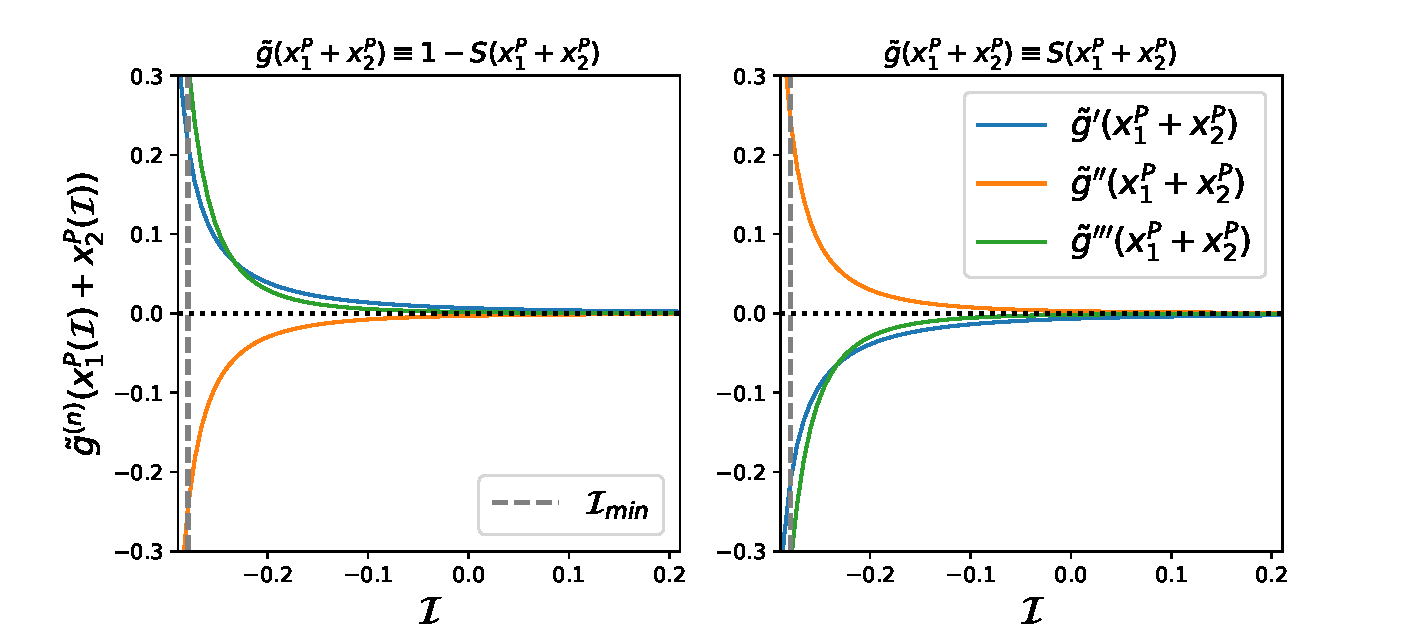
\includegraphics[scale=0.6]{figs/numerics/satfff_derivatives_g.pdf}
    \caption{Higher-order derivatives of $\tilde{g}(x_1^P + x_2^P)$ as functions of the input 
    parameter $\mathcal{I}$.}
    \label{fig:sat_ex1}
\end{figure}
